%\section{Independent Certificate Chains}
%\label{sec:independence}

%In \autoref{sec:design:policy} we describe how we can use a graph of certificate
%fingerprints to compute the policy value for a domain. Specifically, we compute
%the policy value as the minimum number of \ac{ca} private keys that would need
%to be compromised to create an independent set of certificate chains for an
%adversary's public key. However, this value does not necessarily result in truly
%independent certificate chains, as many \acp{ca} control multiple private keys.
%If a single \ac{ca} with poor issuance practices possesses multiple private
%keys, an adversary may gain fraudulent certificates from multiple private keys
%in a single attack. If these certificates are in multiple independent chains,
%then an adversary may be able to mount \iac{mitm} attack.

%One solution to this vulnerability is to use the certificate's issuer
%organization name to differentiate \acp{ca}, but the success of this approach
%depends on the \ac{ca} itself. As we describe in
%\autoref{sec:evaluation:updates}, we found certificates that are likely from the
%same issuer, but have slightly different issue organization names. Furthermore,
%one \acp{ca} may own another and use similar security practices. If these
%\acp{ca} do not certify one another, their certificate chains may be considered
%independent by log aggregators. While we leave deeper exploration of this area
%to future work, we can easily configure \ac{name} to determine the independence
%of certificate chains by the issuer key or organization name, and this is likely
%to provide sufficient security for the vast majority of cases.

%\section{Certificate Issuance Trends}
%\label{sec:certificates}

%In \autoref{sec:evaluation:https}, we computed the set of domain names that
%could potentially\footnote{we say ``potentially'' here because as we point out
%in \autoref{sec:evaluation:https}, the presence of a certificate does not
%necessarily mean the name is publicly reachable via \ac{https}.} deploy
%\ac{https} over time. We extracted this by computing an ``active set'' of
%certificates on each day between March 26, 2013 and July 3, 2018.

%\begin{figure}
  %\centering
  %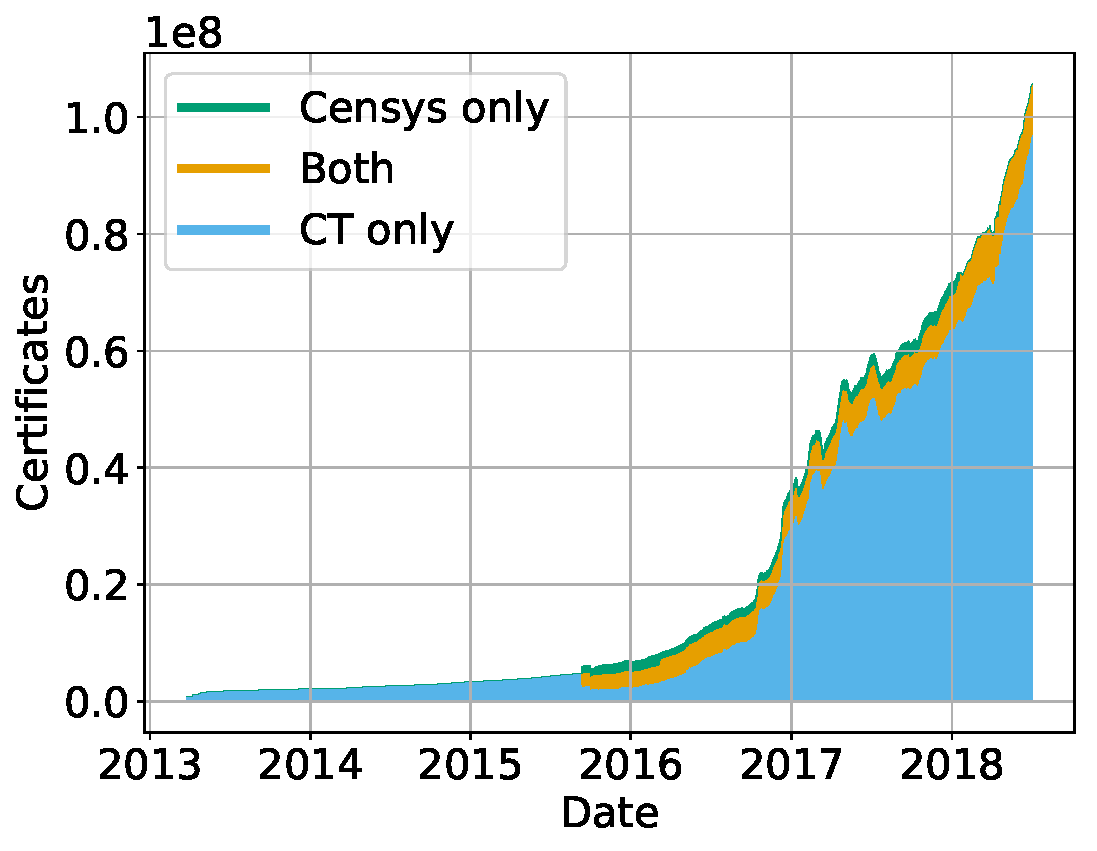
\includegraphics[width=0.8\linewidth]{fig/cert_count_valid}
  %\caption{Number of unique certificates seen by Censys and \ac{ct} over time.}
  %\label{fig:certs}
%\end{figure}

%\autoref{fig:certs} shows that for the most part, the trend in the number of
%active certificates on a given day matches the trend in the number of active
%domain names as seen in \autoref{fig:count:names}. There does, however, seem to
%be slightly more churn in the number of active certificates over time,
%particularly during 2017, in which the usage of Let's Encrypt was becoming
%increasingly widespread. We point out that the number of names is almost
%consistently greater than the number of certificates due to the fact that
%certificates can contain multiple names (and many popular sites such as Google
%have certificates with all of their domain names).

\section{Updates to the Signaling Set}
\label{sec:updates}

In \autoref{sec:evaluation:updates}, we showed that the size of updates to the
signaling set were slowly increasing over time. To better understand how the
size of the signaling set may change over time, we also considered the additions
and deletions to the signaling set separately.

\begin{figure}[t]
  \centering
  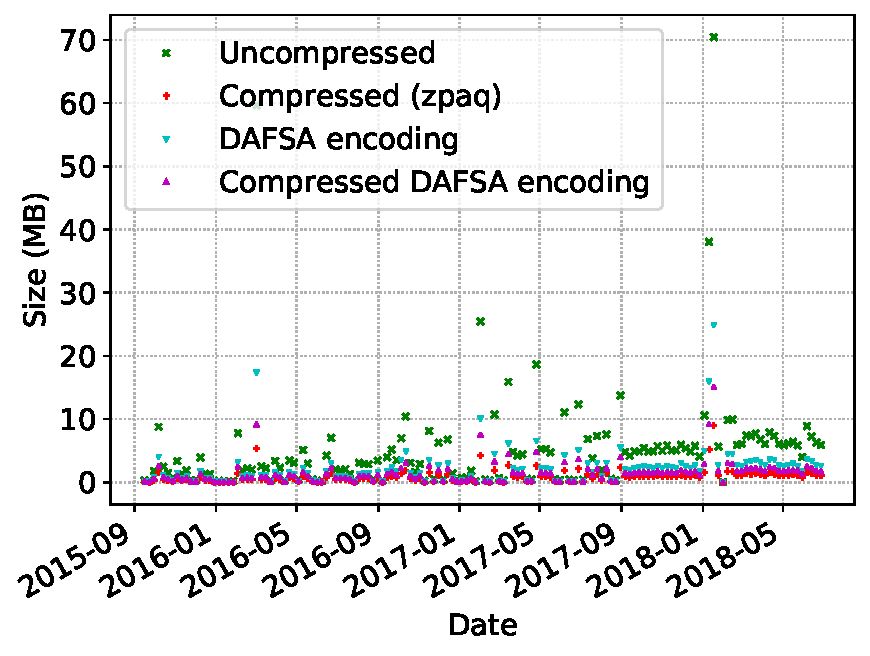
\includegraphics[width=0.95\linewidth]{fig/added_name_set_size}
  \caption{Sizes of the set of added names over time in different
  representations.}
  \label{fig:updates:added}
\end{figure}

\begin{figure}[t]
  \centering
  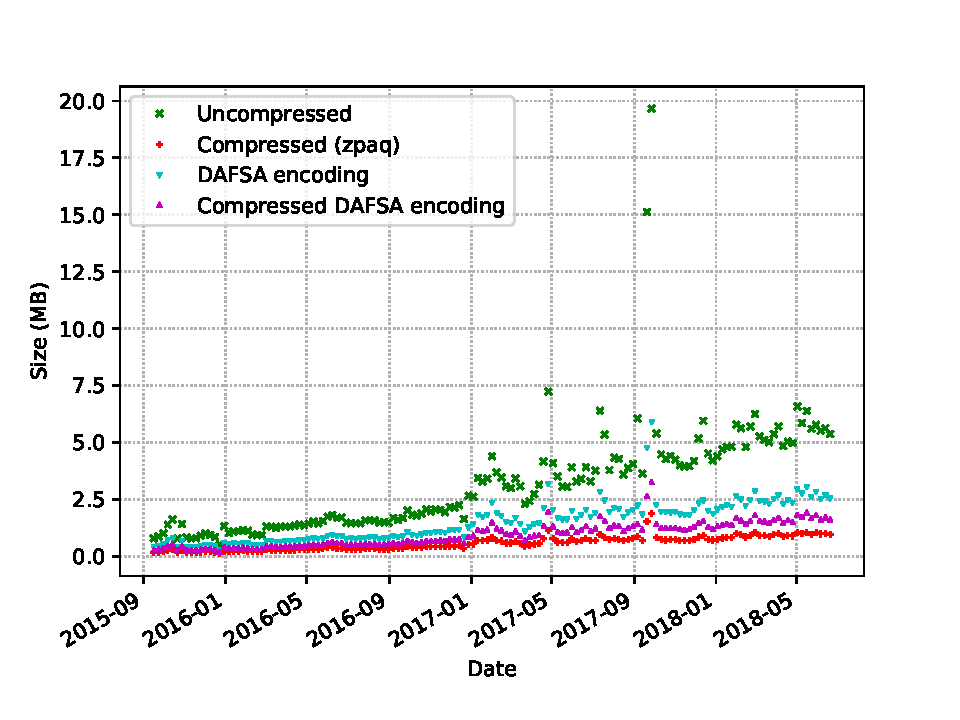
\includegraphics[width=0.95\linewidth]{fig/deleted_name_set_size}
  \caption{Sizes of the set of deleted names over time in different
  representations.}
  \label{fig:updates:deleted}
\end{figure}

Figs.~\ref{fig:updates:added} and~\ref{fig:updates:deleted} show the sizes of
these sets over time. We see that the set of added names is almost consistently
larger than the set of deleted names, which matches the upward trend in the
number of domain names in the Web \ac{pki} over time. We also note that
beginning in 2017, in which Let's Encrypt issuance became more widespread, that
the number of deleted names begins to trend upwards at a greater rate. This is
likely due to the fact that Let's Encrypt certificates are issued for only 90
days at a time, and the increased frequency in certificate expiration causes
names to be purged from the active set at a greater rate.

\begin{figure}[t]
  \centering
  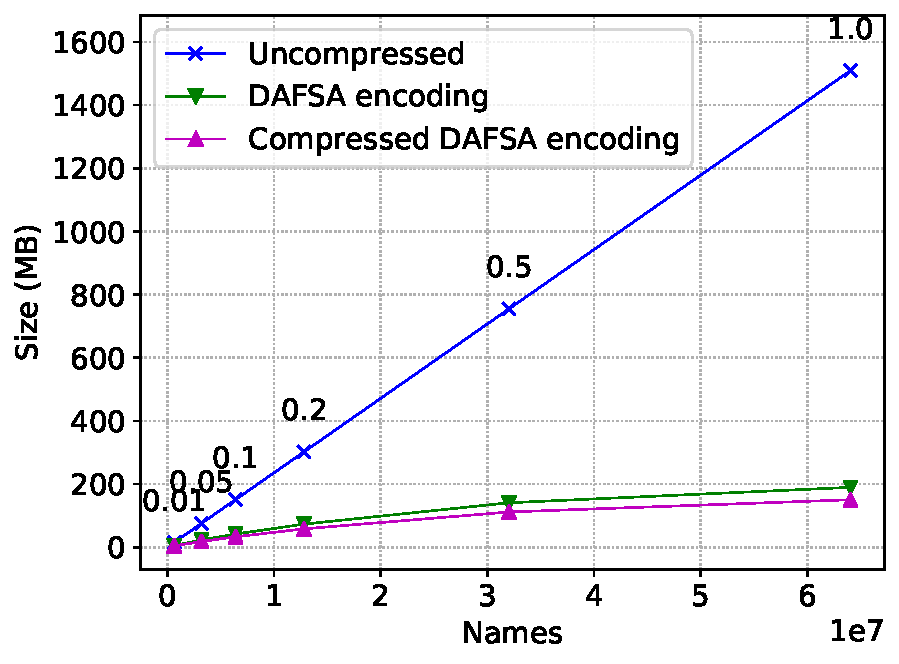
\includegraphics[width=0.95\linewidth]{fig/sample}
  \caption{Size of the signaling set given subsampling from the full set of
  names. The labels above each distinct value on the $x$-axis denote the
fraction of the full set that was sampled.}
  \label{fig:sample}
\end{figure}

Despite the increase in the number of names (and hence in the size of the
signaling set) over time, we argued in \autoref{sec:discussion} that this
increase would be outweighed by the sublinear growth of the signaling set size
and falling cost of storage and memory. We can see the trend in the signaling
set size especially well in \autoref{fig:sample}, a graphical representation of
\autoref{tab:sample}.

\section{Detailed Performance Measurements}
\label{sec:overhead}

\begin{figure}[t]
  \centering
  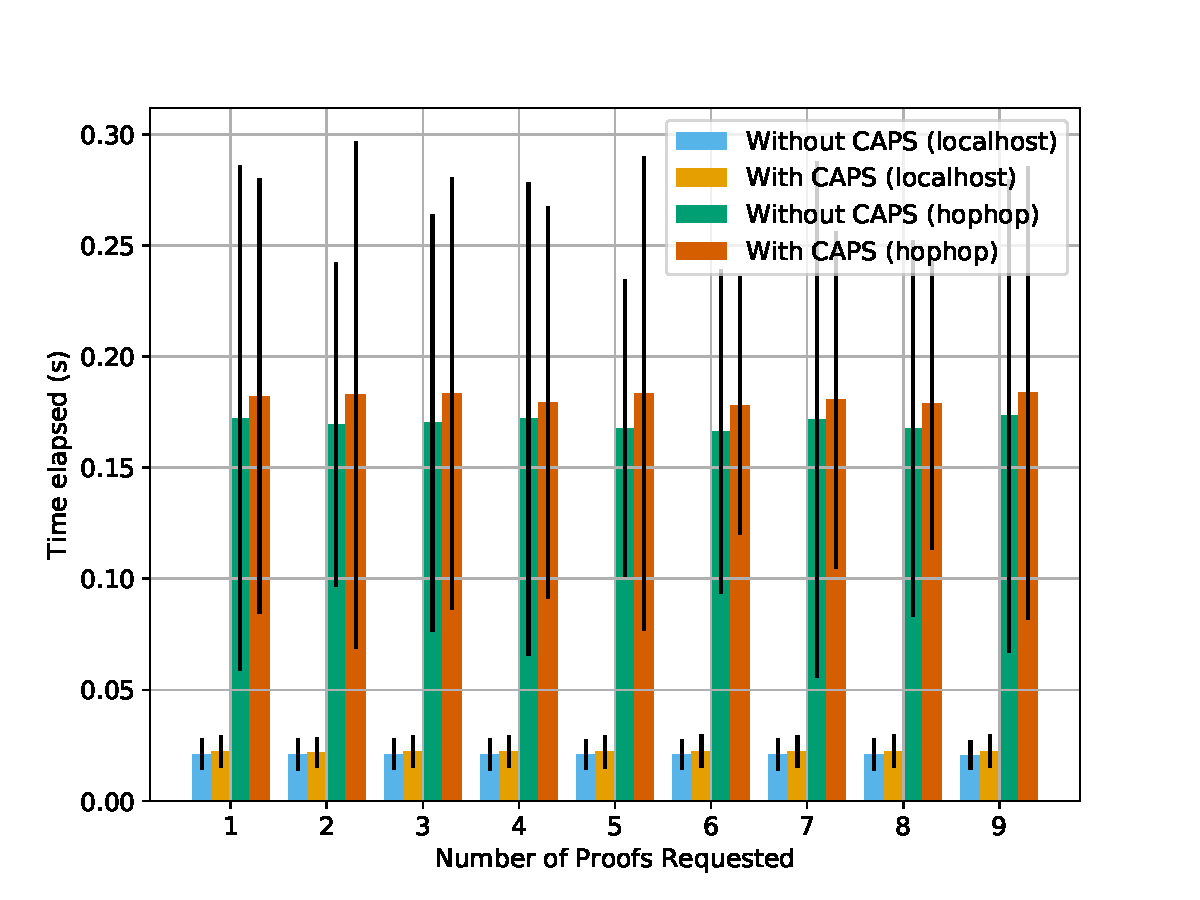
\includegraphics[width=0.8\linewidth]{fig/eval_tls_ext/0-time_elapsed_vs_num_proofs_requested}
  \caption{Handshake latency versus the number of policy proofs sent by the
  domain. Error bars represent standard error.}
  \label{fig:numproofs}
\end{figure}

\begin{figure}[t]
  \centering
  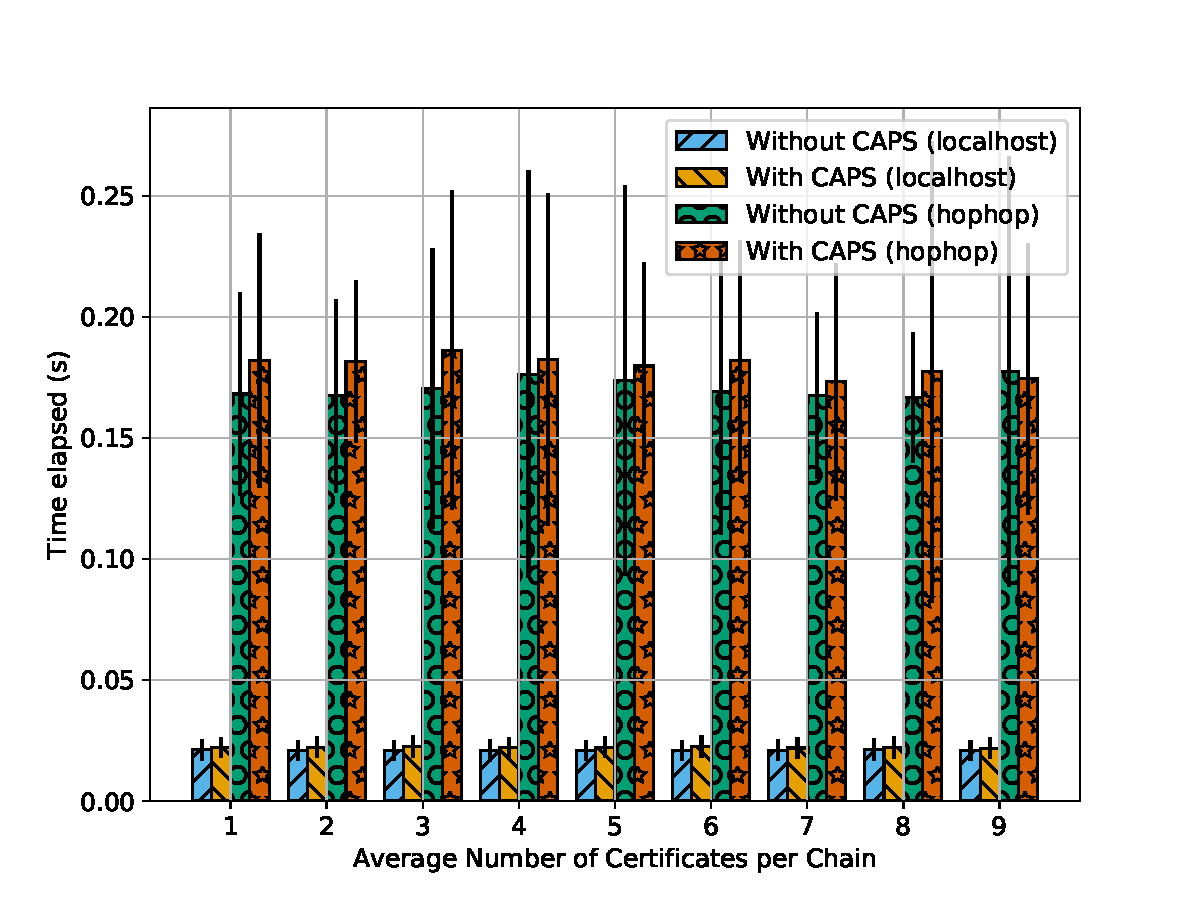
\includegraphics[width=0.8\linewidth]{fig/eval_tls_ext/2-time_elapsed_vs_num_certs_per_chain}
  \caption{Handshake latency versus the number of certificates per chain sent by the
  domain. Error bars represent standard error.}
  \label{fig:numcerts}
\end{figure}

\begin{figure}[t]
  \centering
  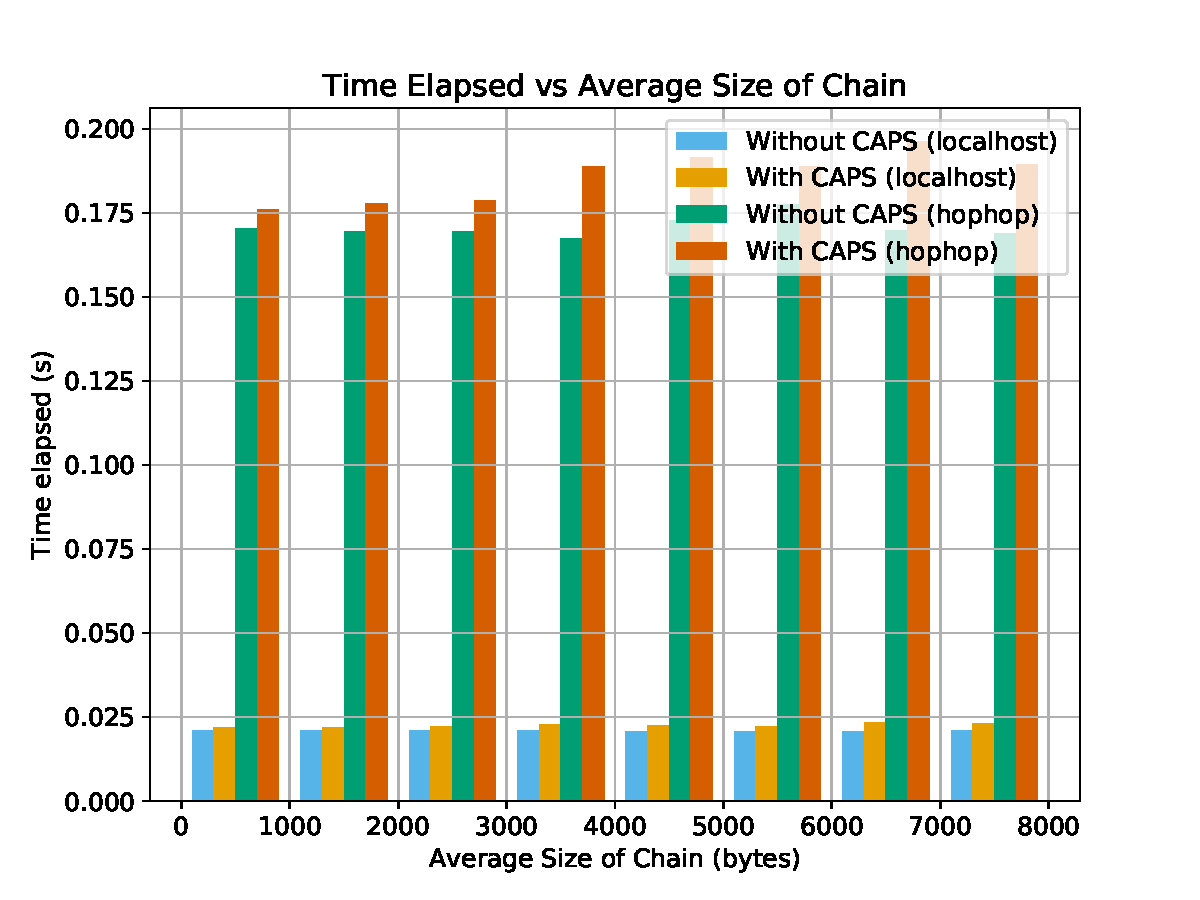
\includegraphics[width=0.8\linewidth]{fig/eval_tls_ext/3-time_elapsed_vs_avg_chain_size}
  \caption{Handshake latency versus the average certificate chain size sent by the
  domain. Error bars represent standard error.}
  \label{fig:chainsize}
\end{figure}

In \autoref{sec:evaluation:performance}, we showed that the connection latency
overhead in using \ac{name} is approximately 5\%. Figs.~\ref{fig:numproofs},
\ref{fig:numcerts}, and~\ref{fig:chainsize} show this overhead given the number
of policy proofs request, the number of certificates per chain, and the average
size of each certificate chain, respectively. In almost every case, the variance
in network latency resulted in error bars that far exceed the difference in
latency between using the existing Web \ac{pki} and using \ac{name}.

Given the way we structured the messages in our \ac{name} \ac{tls} extension,
the extra data sent in the \ac{name} handshake is directly dependent on the size
and number of certificate chains, as well as the number of proofs sent. In
particular, the extra data sent from client to server is 1 byte, and the extra
data sent from server to client is $(2 + (292 \times \text{\#proofs}) +
(\sum_{\text{chain}}\texttt{sizeof}(\text{chain})))$ bytes. 
